\documentclass{beamer}
\usepackage{tikz}

\definecolor{mh_bg}{HTML}{f6f6f6}
\definecolor{mh_main}{HTML}{6495ED} % cornflowerblue

\beamertemplatenavigationsymbolsempty
\setbeamercolor*{structure}{fg=mh_main}
\setbeamercolor{block title}{use=structure,fg=black,bg=mh_bg}
\setbeamercolor{block body}{parent=normal text,use=block title,bg=mh_bg!25}
\setbeamertemplate{blocks}[rounded][shadow=true]
\setbeamerfont{block title}{size=\small}

\usepackage{listings}
\lstset{basicstyle=\scriptsize\tt}
\lstset{keywordstyle=\scriptsize\tt\color{mh_main}}
\lstset{commentstyle=\scriptsize\tt\color{black!60}}

\newcommand{\mh}[0]{{\sc\structure{Miss\_Hit}}}
\newcommand{\matlab}[0]{MATLAB\textsuperscript{\tiny\textregistered}}
\newcommand{\simulink}[0]{Simulink\textsuperscript{\tiny\textregistered}}

\author{Florian Schanda}
\title{What is {\sc Miss\_Hit}?}
\subtitle{A quick overview}
\date{April 23, 2020}

\begin{document}

\maketitle

\setbeamertemplate{background}
{
\begin{tikzpicture}[overlay]
    \fill[mh_bg] (0, 0) rectangle (\paperwidth, -\paperheight);
    \fill[mh_bg!50] (0.45, -\paperheight) [rounded corners] --
                       (0.45, -1.45) [sharp corners] --
                       (\paperwidth, -1.45) --
                       (\paperwidth, -\paperheight) --
                       cycle;
    \fill[white] (0.5, -\paperheight) [rounded corners] --
                 (0.5, -1.5) [sharp corners] --
                 (\paperwidth, -1.5) --
                 (\paperwidth, -\paperheight) --
                 cycle;
\end{tikzpicture}}

\section{Overview}
\begin{frame}{Overview}
  \mh~is:
  \begin{itemize}
  \item A free-software compiler framework for the full \matlab\
    language and most of the GNU Octave language \pause
  \item A supplementary tool-suite for \matlab, \simulink\ and GNU
    Octave
    \begin{itemize}
    \item A \structure{style checker}
    \item A \structure{code formatter}
    \item A \structure{code metric tool}
    \end{itemize}
  \end{itemize}
\end{frame}

\begin{frame}{Availability, License, and Requirements}
  \begin{itemize}
  \item Available on GitHub: \url{https://github.com/florianschanda/miss_hit}
  \item Licensed under GPLv3
    \pause
  \item Requires only Python 3.6+
  \item Does \emph{not} require a working \matlab\ or GNU Octave
    environment
  \end{itemize}
\end{frame}

\section{Tools}
\subsection{Style Checker}
\begin{frame}{Tool overview}{Style checker}
  \begin{itemize}
  \item Can check many style issues, e.g:
    \begin{itemize}
    \item Whitespace issues
    \item Indentation
    \item Naming of variables, functions, classes
    \item etc.
    \end{itemize}
  \item Highly configurable through config files
  \item Justification mechanism for messages
  \end{itemize}
\end{frame}

\begin{frame}[fragile]{Tool overview}{Style checker}
  \begin{block}{Example code}
\begin{lstlisting}[language=MATLAB]
if (foo)
\end{lstlisting}
  \end{block}
  \pause
  \begin{block}{Output of {\tt mh\_style.py}}
    \scriptsize
\begin{verbatim}
In test.m, line 7
| if (foo)
|    ^ style: redundant parenthesis
\end{verbatim}
  \end{block}
\end{frame}

\begin{frame}{Tool overview}{Code formatter}
  \begin{itemize}
  \item Almost all issues can be automatically fixed
  \item Just use the {\tt --fix} option
  \end{itemize}
\end{frame}

\begin{frame}[fragile]{Tool overview}{Code formatter}
  \begin{block}{Example code}
\begin{lstlisting}[language=MATLAB]
function rv= foo (x), if x < 0,,rv=-   x;else,rv=x;,; end;
\end{lstlisting}
  \end{block}
  \pause
  \begin{block}{Fixed code using {\tt mh\_style.py --fix}}
\begin{lstlisting}[language=MATLAB]
function rv = foo (x)
    if x < 0
        rv = -x;
    else
        rv = x;
    end
\end{lstlisting}
  \end{block}
\end{frame}

\begin{frame}[fragile]{Tool overview}{Code formatter}
  Code formatter is fully aware of all whitespace peculiarities!
  \pause
  \begin{center}
    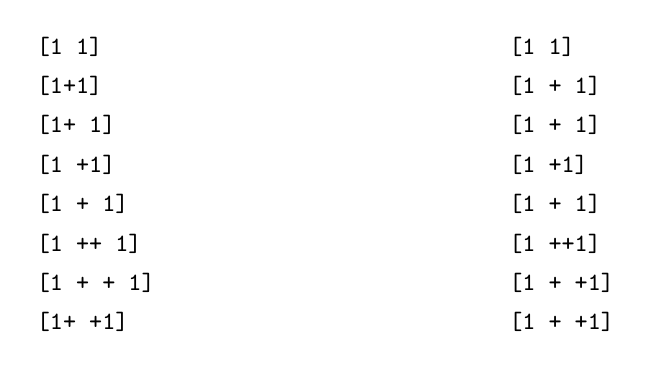
\begin{tikzpicture}[y=-0.5cm,x=3cm,font=\tt\small]
      \node[anchor=west] at (0, 0) {[1 1]};     % [1 1]
      \node[anchor=west] at (0, 1) {[1+1]};     % [2]
      \node[anchor=west] at (0, 2) {[1+ 1]};    % [2]
      \node[anchor=west] at (0, 3) {[1 +1]};    % [1 1]
      \node[anchor=west] at (0, 4) {[1 + 1]};   % [2]
      \node[anchor=west] at (0, 5) {[1 ++ 1]};  % [1 1]
      \node[anchor=west] at (0, 6) {[1 + + 1]}; % [2]
      \node[anchor=west] at (0, 7) {[1+ +1]};   % [2]

      \visible<3->{
      \node[anchor=west] at (2, 0) {[1 1]};
      \node[anchor=west] at (2, 1) {[1 + 1]};
      \node[anchor=west] at (2, 2) {[1 + 1]};
      \node[anchor=west] at (2, 3) {[1 +1]};
      \node[anchor=west] at (2, 4) {[1 + 1]};
      \node[anchor=west] at (2, 5) {[1 ++1]};
      \node[anchor=west] at (2, 6) {[1 + +1]};
      \node[anchor=west] at (2, 7) {[1 + +1]};
      }
    \end{tikzpicture}
  \end{center}
  \pause
  All of this works correctly!
\end{frame}

\subsection{Code Metrics}
\begin{frame}{Tool overview}{Code metric tool}
  \mh~also includes a code metric tool that can measure:
  \begin{itemize}
  \item Cyclomatic complexity (equivalent to {\tt mlint -cyc})
  \item Path count
  \item Maximum nesting of control structures
  \item Number of function parameters
  \item Number of global variables
  \item Number of persistent variables
  \item Line count for each function
  \end{itemize}
  \pause
  Also works for embedded code inside \simulink\ models!
\end{frame}

\begin{frame}{Tool overview}{Code metric tool}
  HTML report is probably the most useful:
  \begin{center}
    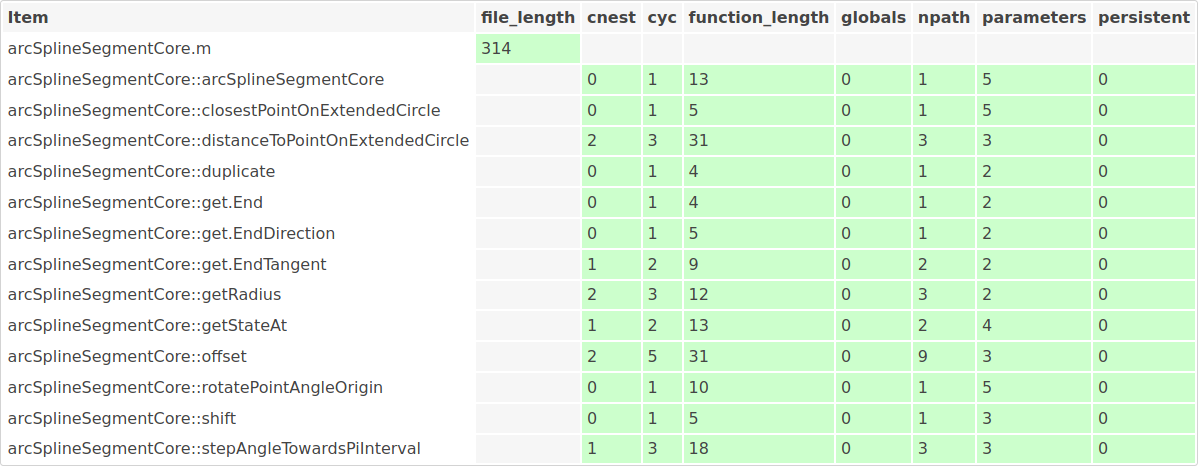
\includegraphics[width=10cm]{metrics.png}
  \end{center}
\end{frame}

\begin{frame}[fragile]{Tool overview}{Code metric tool}
  Exceeding metric generates messages:
  \begin{block}{Example}
    \scriptsize
\begin{verbatim}
In function_file.m, line 3
| function function_file
|          ^^^^^^^^^^^^^ metric: exceeded npath: measured 8 > limit 5
\end{verbatim}
  \end{block}
\end{frame}

\begin{frame}[fragile]{Tool overview}{Code metric tool}
  Justification mechanism allows you to locally exceed limits:
  \begin{block}{Justification pragma example}
\begin{lstlisting}[language=MATLAB]
function function_file_justified
  %| pragma Justify(metric, "npath",
  %|                "this is fine for reasons...");
  if rand() > 0.5
    disp heads;
  else
    disp tails;
  end

  % ...
\end{lstlisting}
  \end{block}
  \pause
  Justification is included in report.
\end{frame}

\begin{frame}{Optimised for CI}
  \mh~is ideal for integration in your continuous integration
  environment:
  \begin{itemize}
  \item Low foot-print, no requirements (only Python 3)
  \item Multi-threaded analysis
  \item Justification mechanism allows you to maintain code metrics
    and style on every commit
  \item When it comes to ``release'' time, you just need to generate
    reports and you're done
  \end{itemize}
\end{frame}

\section{Conclusion}
\subsection{Getting Help}
\begin{frame}{Getting help}
  \begin{itemize}
  \item Documentation describes everything: style rules, metrics, and
    how to use the configuration files
  \item \url{https://florianschanda.github.io/miss_hit/}
    \pause
  \item Found a bug / want something done? Raise an issue on GitHub!
  \end{itemize}
\end{frame}

\subsection{Roadmap}
\begin{frame}{Roadmap}
  Some ideas for the future:
  \begin{itemize}
  \item Linter tool
    \begin{itemize}
    \item Semantic analysis
    \item Data and information flow analysis
    \end{itemize}
  \item More GNU Octave support
  \item GNU Octave / \matlab\ compatibility check
  \item Tool qualification for e.g. ISO 26262
    \pause
  \item \structure{Anything else users suggest!}
  \end{itemize}
\end{frame}

\subsection{Summary}
\begin{frame}{Conclusion}
  \begin{itemize}
  \item \mh~is the only free-software parser for full \matlab\ I'm
    aware of
  \item Works for code embedded in \simulink\ models
  \item Fills holes in the \matlab\ eco-system
    \begin{itemize}
    \item Reliable code formatting
    \item Metrics
    \end{itemize}
  \item Built on solid foundations so more features will come
  \end{itemize}

  \vspace{12pt}

  \visible<2->{
    \begin{center}
      \structure{Thank you for your time and attention.}\\
      {\scriptsize Made using only Free Software}
    \end{center}
  }
\end{frame}

\end{document}
